\documentclass[tikz,margin=5]{standalone}

\usepgfmodule{nonlineartransformations}
\usepgflibrary{curvilinear}
\usetikzlibrary{spy}
\usetikzlibrary{calc}

\tikzset{pics/grid/.style={code={%
	\tikzset{x=10pt, y=10pt, step=10pt}
	\draw [thin] (-2, 0) grid ++(4, 20);
	\draw [thick] (-2, 0)
		rectangle ++(4, 20) (-4, 0) -- (4, 0);
	\draw [thick, fill=gray!50] (0, 14)
		rectangle ++(1,1) ++(-.5,-.5) coordinate (-square);
	\draw [<->, thin, gray] (0, 14) -- ++(1, 1);
	\coordinate (-corner) at (-2, 20);
}}}

\begin{document}

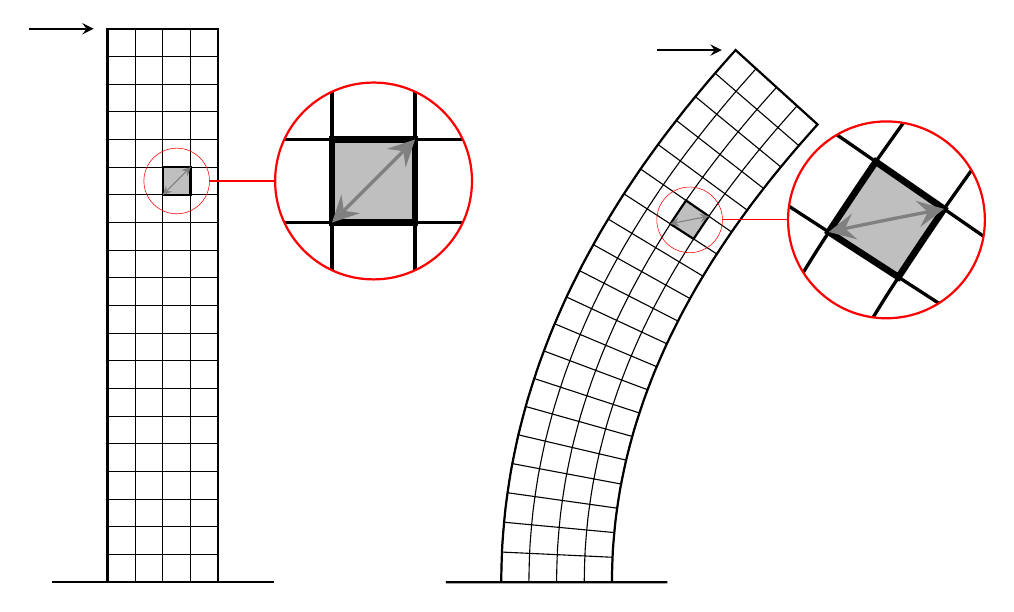
\begin{tikzpicture}[>=stealth, spy using outlines={circle, magnification=3, size=2.5cm, connect spies}]

\pic (a) {grid};
\draw [->, thick, shorten >=5] (a-corner) ++(-1,0) -- (a-corner);
\spy [red] on (a-square) in node at ($ (a-square)+(2.5,0) $);

\scoped{
	\pgfsetcurvilinearbeziercurve
		{\pgfpointxy{5}{0}}{\pgfpointxy{5}{10}}
		{\pgfpointxy{25}{15}}{\pgfpointxy{25}{20}}
	\pgftransformnonlinear{\pgfgetlastxy\x\y%
		\pgfpointcurvilinearbezierorthogonal{\y}{-\x}}%
	\pic (b) {grid};
}

\draw [->, thick, shorten >=5] (b-corner) ++(-1, 0) -- (b-corner);
\spy [red] on (b-square) in node at ($ (b-square) + (2.5, 0) $);

\end{tikzpicture}

\end{document}
